%
% cre.tex (LateX)
% 
% Objetivo: Capítulo sobre o método CRE do relatório de qualificação de doutorado.
% 
% Versão 1.0
% 
% Site: http://www.dirackslounge.online
% 
% Programador: Rodolfo A. C. Neves (Dirack) 07/10/2019
% 
% Email: rodolfo_profissional@hotmail.com
% 
% Licença: GPL-3.0 <https://www.gnu.org/licenses/gpl-3.0.txt>.

\chapter{EMPILHAMENTO ELEMENTO DE REFLEXÃO COMUM (ERC)}
\label{cap2:cre}

O método empilhamento Elemento de Reflexão Comum (ERC) é uma alternativa para os métodos de empilhamento PMC ou
migração para a seção de afastamento nulo. Não requer conhecimento do modelo geral em subsuperfície, apenas
o conhecimento da velocidade próxima a superfície é necessário a priori.
O método ERC é baseado somente em considerações cinemáticas 2D e não é
um processo que preserva as amplitudes.
A principal vantagem do método ERC em comparação com o empilhamento PMC convencional
é que este proporciona a seção empilhada e parâmetros importantes para a construção do macromodelo de 
velocidades que pode inclusive variar lateralmente \cite{cre}.

As principais características do método ERC são:
\begin{enumerate}
 \item[(a)] A construção da seção de afastamento nulo a partir de um conjunto de seções de afastamento constante
com apenas uma estimativa da velocidade próxima da superfície.

 \item[(b)] A determinação dos parâmetros $(R_{NIP},\beta_0)$ para as reflexões de afastamento nulo na seção empilhada.
Estes atributos podem ser utilizados com técnicas de inversão para estimar o macromodelo de velocidades.
\end{enumerate}

Os parâmetros $R_{NIP}$ e $\beta_0$ 
são atributos específicos de uma frente de onda hipotética atribuídos a cada evento de reflexão
primária de afastamento nulo: O raio de curvatura $R_{NIP}$ e o ângulo de emergência $\beta_0$. Esta onda hipotética é
a onda NIP \cite{hubral}.

A idéia principal do método ERC é usar a fórmula do tempo de trânsito ERC no modelo auxiliar para
encontrar a frente de onda NIP que melhor se ajusta aos dados, dado um intervalo
de busca para os parâmetros $R_{NIP}$ e $\beta_0$,
Este processo é semelhante a análise sobretempo normal convencional, todavia enquanto esta análise é feita no
domínio PMC, o método ERC é feito no domínio ERC construído durante o processo. Os parâmetros otimizados $R_{NIP}$ e $\beta_0$
são especificados a partir da análise de coerência nos dados \cite{cre}.

As coordenadas das curvas ERC, mesmo sem o conhecimento da curvatura do refletor em subsuperfície, são definidas
a partir dos parâmetros $R_{NIP}$ e $\beta_0$, obtidos através de um processo de otimização, 
para cada PMC central $m_0$ na seção de afastamento nulo. A Equação que descreve a trajetória ERC no plano $m, h$ \cite{cre}:

\begin{equation}
 \label{eq:2.1}
 m= m_0 + \frac{1}{2\alpha} (1-\sqrt{1+4\alpha^2h^2})
\end{equation}

Onde $\alpha$ é um parâmetro de assimetria que desenpenha um papel importante na seleção de pares fonte-receptor para os quais
os correspondentes raios de reflexão incidem no mesmo ponto sobre o refletor \cite{tygel}. E é dado por:

\begin{equation}
\label{eq:2.2}
 \alpha=\frac{\sin{\beta_0}}{R_{NIP}}
\end{equation}

Os traços sísmicos com as coordenadas $m, h$ dadas pela Equação \ref{eq:2.1} formam uma família ERC.
O método ERC também possui uma aproximação de tempo de trânsito de
reflexão \cite{cre}:

\begin{multline}
\label{eq:2.3}
t(m,h)= \left( \tau_0-\frac{2R_{NIP}}{v_0} \right) 
+\frac{R_{NIP}}{v_0}\sqrt{1-2\alpha(m-m_0+h)+\frac{(m-m_0+h)^2}{R_{NIP}^2}} \\
+\frac{R_{NIP}}{v_0}\sqrt{1-2\alpha(m-m_0-h)+\frac{(m-m_0-h)^2}{R_{NIP}^2}}
\end{multline}

Onde $t(m,h)$ é o tempo de trânsito de reflexão no domínio ERC para o PMC $m$ e o meio afastamento $h$.
$v_0$ é a velocidade próxima da superfície, $\tau_0$ é o tempo de trânsito de afastamento nulo e 
$R_{NIP}$ e $\alpha$ são os parâmetros otimizados associados a um PMC central $m_0$. A derivação da
Equação \ref{eq:2.3} é apresentada em detalhes no Apêndice \ref{ap:tempo_cre}.

A Equação \ref{eq:2.3} é utilizada para o empilhamento no domínio ERC. As amostras nas famílias ERC 
que estão sobre esta curva de tempo de trânsito são empilhadas e atribuídas ao PMC central $m_0$ na seção empilhada.
Ao realizar este processo para todos os $m_0$'s da malha obtemos a imagem na seção empilhada ERC.

\begin{figure}[H]
\caption{Representação esquemática de um arranjo ERC para um refletor circular de raio $R$ e profundidade
mínima $D$: A família ERC é formada pelos pares $s_i$-$r_i$ (fonte-receptor) que possuem o mesmo ponto de
reflexão em subsuperfície (ponto $NIP$). A família ERC pode ser entendida a partir de uma fonte pontual explosiva
no ponto $NIP$, que ao ser ativada forma uma frente de onda $NIP$ que atinge a superfície em um PMC central 
$m_0$ com raio de curvatura $R_{NIP}$ e ângulo de incidência $\beta_0$.}
\begin{center}
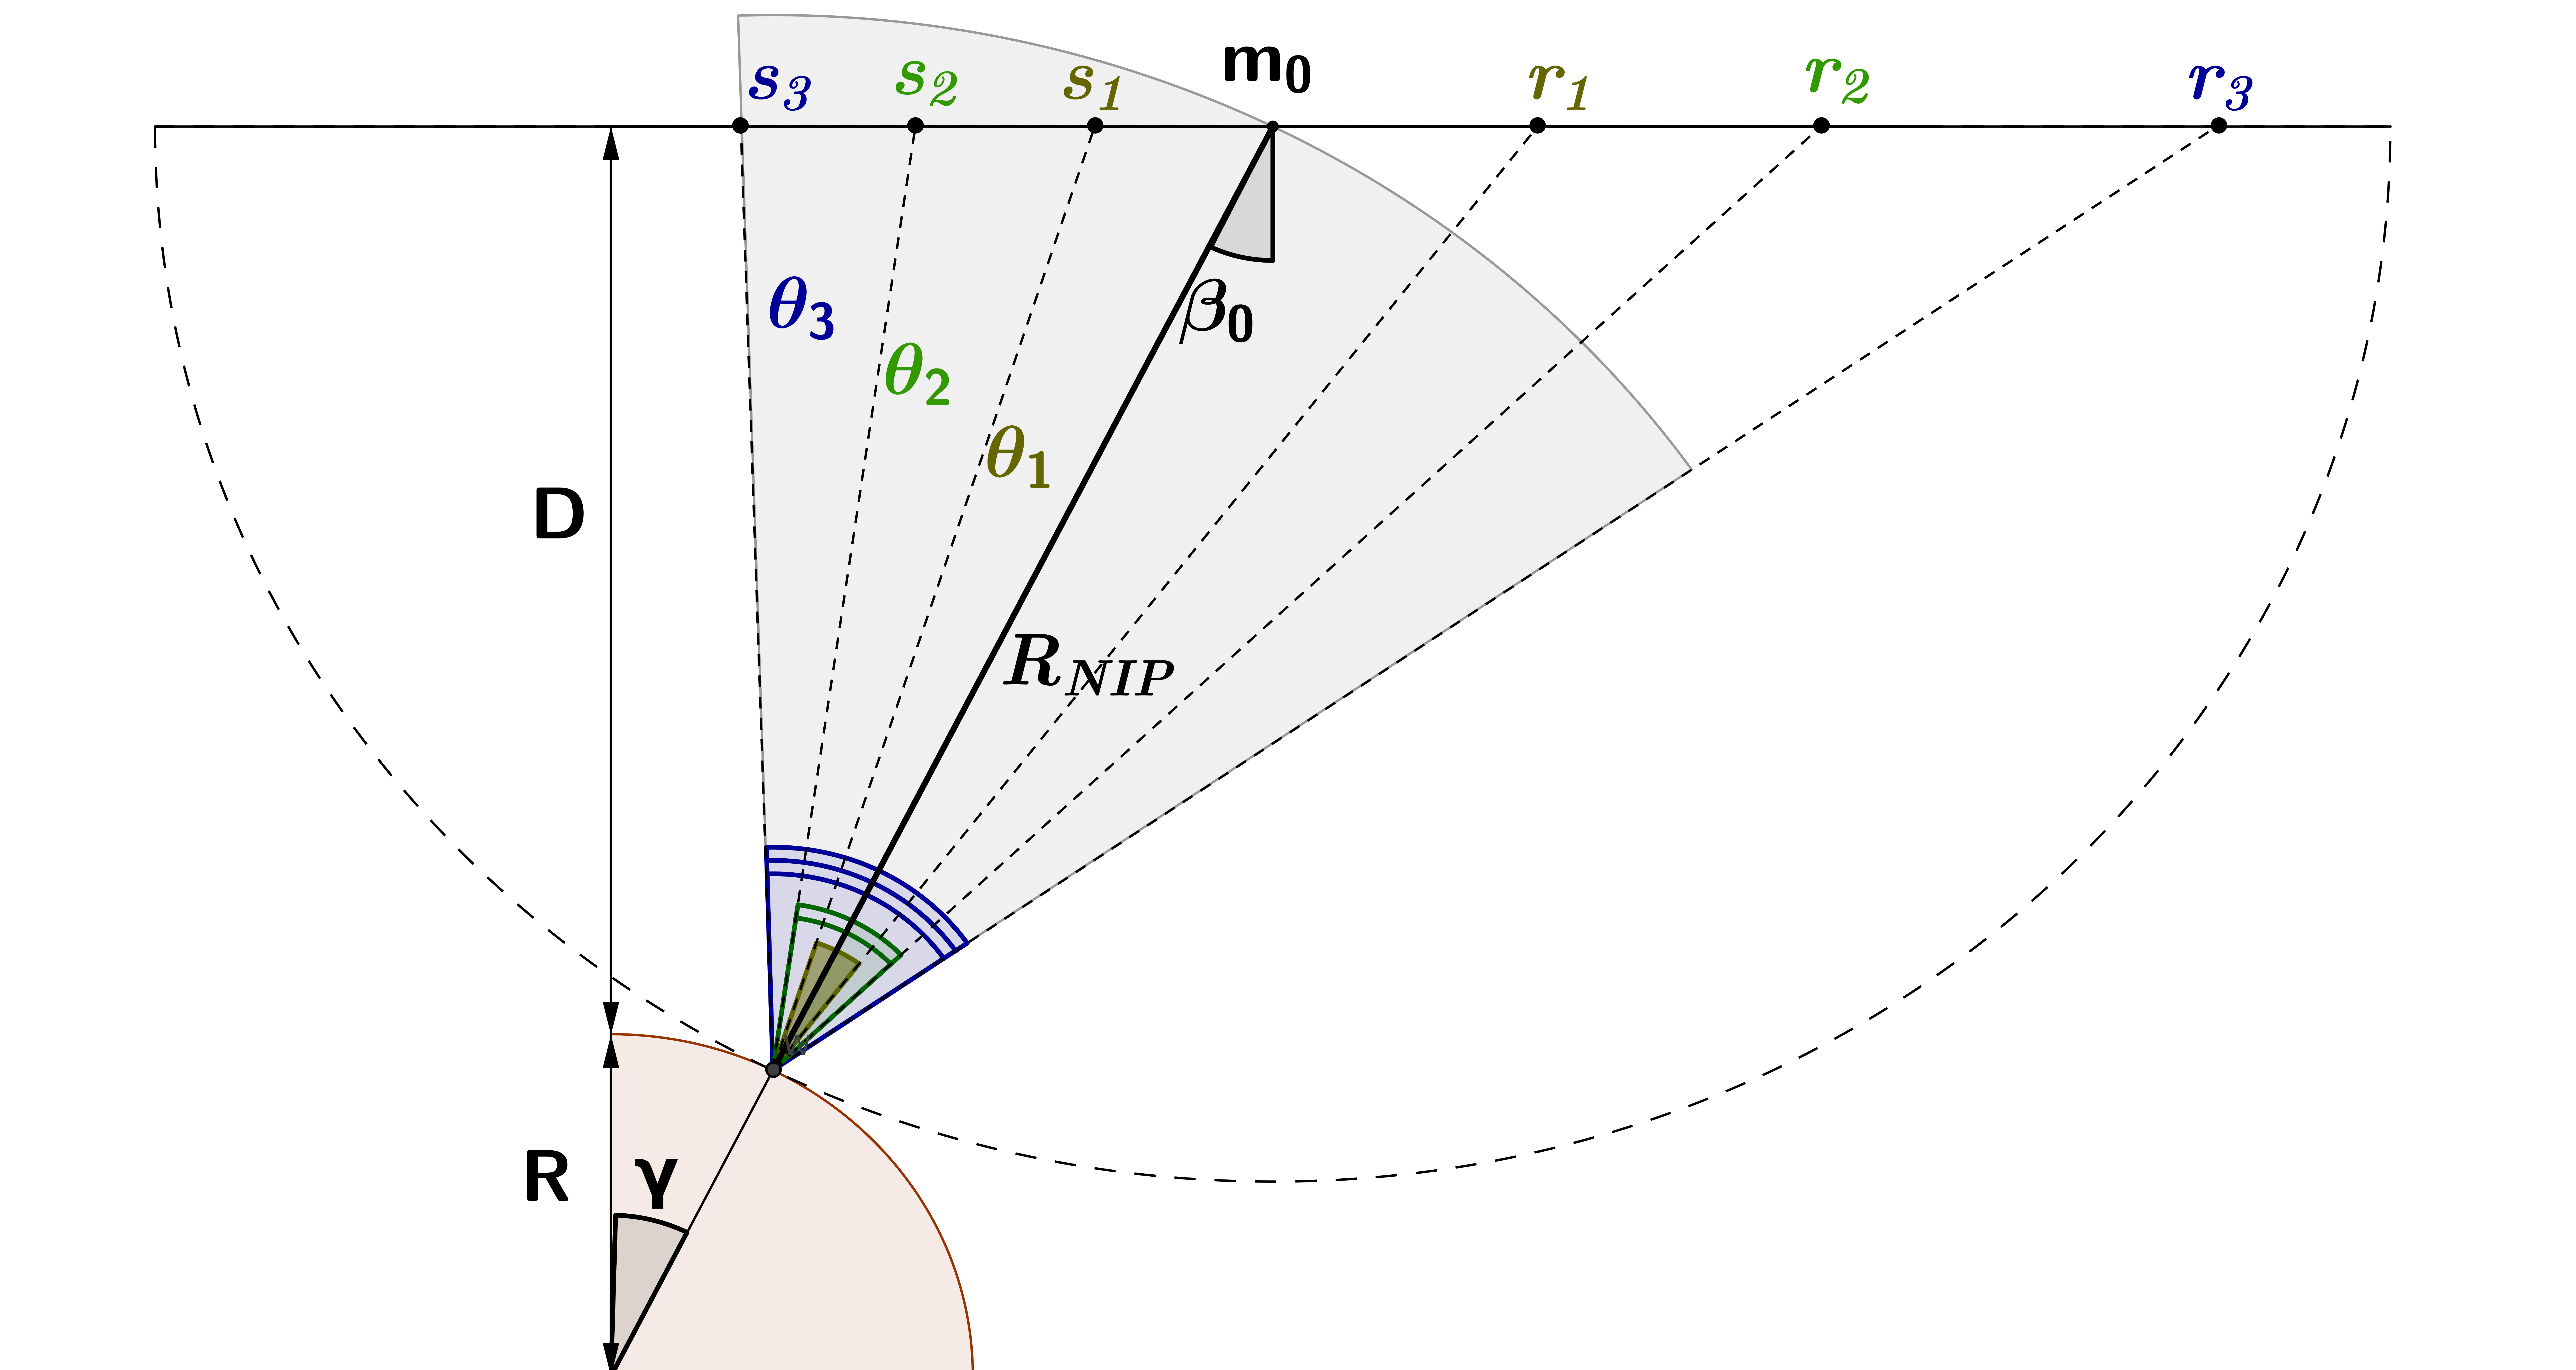
\includegraphics[scale=0.3]{images/cre.png}
\vspace{-0.3cm}
\end{center}
\begin{center}
 Fonte: Do Autor.
\end{center}
\label{fig:2.1}
\end{figure}

O principal desvantagem do método ERC é que as coordenadas de fontes e receptores são distribuídas assimetricamente em tal 
arranjo: Na Figura \ref{fig:2.1} representamos um arranjo ERC em um modelo do refletor circular 
em um meio com velocidade constante $v$.
Todos os raios de reflexão que saem das fontes $s_i$ e chegam aos receptores $r_i$ 
possuem o mesmo ponto de reflexão sobre o refletor.
Porém, a curvatura do refletor estabelece uma distribuição assimétrica dos pares fonte e receptor no domínio do afastamento $h$
e na distância em relação ao PMC central $m_0$, dada por $d=m-m_0$.

A Figura \ref{fig:2.2} mostra as coordenadas $m, h$ de várias curvas ERC hipotéticas com $\alpha$ dado pela Equação \ref{eq:2.2}.
As curvas ERC intersectam as seções de afastamento constante (linhas horizontais na figura) e as seções de ponto médio comum 
(linhas verticais na figura), não sendo posível construir uma malha regular para amostrar tais curvas simultaneamente nos dois
eixos.
A única distribuição que pode ser amostrada regularmente no plano $m, h$ ocorre quando $\alpha=0$. Esta é
a família de ponto médio comum do PMC $m_0$ (linha vertical com pontos em roxo na figura).

\begin{figure}[htb]
\caption{Representação esquemática das coordenadas de várias trajetórias ERC sobre o plano PMC $m$ x meio afastamento
$h$. As linhas do grid representam as seções de afastamento constante (linhas horizontais) e seções PMC (linhas verticais).
Estas trajetórias foram construídas variando $\beta_0$, $R_{NIP}$ e $\alpha$  na Equação \ref{eq:2.2}. Quando
$\alpha=0$ a trajetória ERC será a trajetória de uma família PMC para um PMC $m_0$.}
\begin{center}
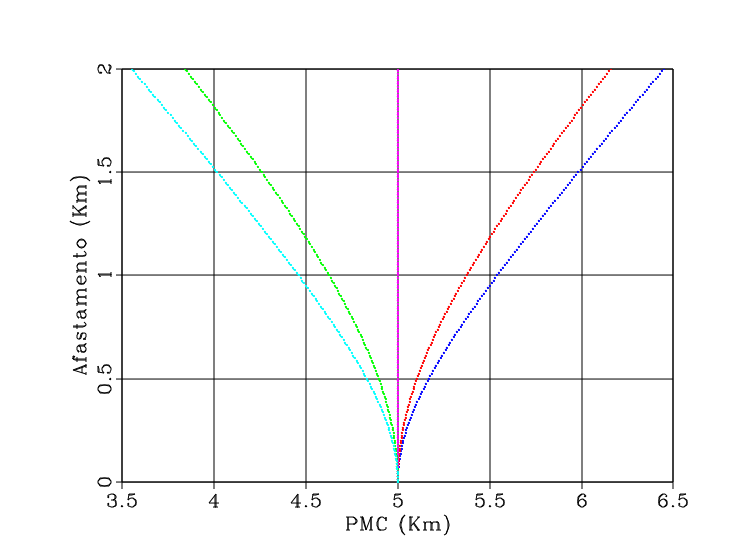
\includegraphics[scale=0.5]{images/creCoord.png}
\vspace{-0.3cm}
\end{center}
\begin{center}
 Fonte: Do Autor.
\end{center}
\label{fig:2.2}
\end{figure}

%% Texto sobre a condição CDS (RN=RNIP)
Neste trabalho propomos uma forma de aumentar a região de convergência da Equação \ref{eq:2.3} utilizando a
aproximação de tempo de trânsito do SRC não hiperbólico e aplicando a condição SDC ($R_N=R_{NIP}$) para
simular a trajetória de tempo de trânsito ERC: No modelo de uma fonte pontual sobre o refletor, o raio de 
curvatura $R_N$ é aproximadamente igual a $R_{NIP}$, esta condição limite é a condição SDC \cite{shav}.

Nossa hipótese é que ao utilizarmos a condição SDC na aproximação de tempo de trânsito do SRC não hiperbólico
teremos uma trajetória de tempo de trânsito ERC com uma região de convergência superior à Equação de tempo de
trânsito ERC (Equação \ref{eq:2.3}).

A aproximação do SRC não hiperbólico possui o
intuito de melhorar a acurácia das aproximações de tempo de trânsito SRC
para grandes afastamentos e separação entre os PMC's \cite{fomel1}.

\begin{equation}
\label{eq:2.4}
 \Phi_{CRS}(h,d;t_0)=\sqrt{\frac{F(d)+ch^2+\sqrt{F(d-h)F(d+h)}}{2}}
\end{equation}

A Equação \ref{eq:2.4} é chamada equação do CRS não-hiperbólico, pois não deriva de uma expansão em série de Taylor
de segunda ordem do tempo de trânsito. Os parâmetros 
$a_1$, $a_2$ e $b_2$
do CRS hiperbólico são utilizados na definição
dos parâmetros do SRC não hiperbólico como \cite{fomel1}:

\begin{equation}
\label{eq:2.5}
 c=2b_2+a_1^2-a_2
\end{equation}

\begin{equation}
\label{eq:2.6}
 F(d-h)=(t_0+a_1(d-h))^2+a_2(d-h)^2
\end{equation}

\begin{equation}
\label{eq:2.7}
 F(d+h)=(t_0+a_1(d+h))^2+a_2(d+h)^2
\end{equation}